%%%%%%%%%%%%%%%%%%%%%%%%%%%%%%%%%%%%%%%%%
% Beamer Presentation
% LaTeX Template
% Version 1.0 (10/11/12)
%
% This template has been downloaded from:
% http://www.LaTeXTemplates.com
%
% License:
% CC BY-NC-SA 3.0 (http://creativecommons.org/licenses/by-nc-sa/3.0/)
%
%%%%%%%%%%%%%%%%%%%%%%%%%%%%%%%%%%%%%%%%%

%----------------------------------------------------------------------------------------
%	PACKAGES AND THEMES
%----------------------------------------------------------------------------------------

\documentclass{beamer}

\mode<presentation> {

% The Beamer class comes with a number of default slide themes
% which change the colors and layouts of slides. Below this is a list
% of all the themes, uncomment each in turn to see what they look like.

%\usetheme{default}
%\usetheme{AnnArbor}
%\usetheme{Antibes}
%\usetheme{Bergen}
%\usetheme{Berkeley}
%\usetheme{Berlin}
%\usetheme{Boadilla}
%\usetheme{CambridgeUS}
%\usetheme{Copenhagen}
%\usetheme{Darmstadt}
%\usetheme{Dresden}
%\usetheme{Frankfurt}
%\usetheme{Goettingen}
%\usetheme{Hannover}
%\usetheme{Ilmenau}
%\usetheme{JuanLesPins}
%\usetheme{Luebeck}
\usetheme{Madrid}
%\usetheme{Malmoe}
%\usetheme{Marburg}
%\usetheme{Montpellier}
%\usetheme{PaloAlto}
%\usetheme{Pittsburgh}
%\usetheme{Rochester}
%\usetheme{Singapore}
%\usetheme{Szeged}
%\usetheme{Warsaw}

% As well as themes, the Beamer class has a number of color themes
% for any slide theme. Uncomment each of these in turn to see how it
% changes the colors of your current slide theme.

%\usecolortheme{albatross}
%\usecolortheme{beaver}
%\usecolortheme{beetle}
%\usecolortheme{crane}
%\usecolortheme{dolphin}
%\usecolortheme{dove}
%\usecolortheme{fly}
%\usecolortheme{lily}
%\usecolortheme{orchid}
%\usecolortheme{rose}
%\usecolortheme{seagull}
%\usecolortheme{seahorse}
%\usecolortheme{whale}
%\usecolortheme{wolverine}

%\setbeamertemplate{footline} % To remove the footer line in all slides uncomment this line
%\setbeamertemplate{footline}[page number] % To replace the footer line in all slides with a simple slide count uncomment this line

%\setbeamertemplate{navigation symbols}{} % To remove the navigation symbols from the bottom of all slides uncomment this line
}

\usepackage{graphicx} % Allows including images
\usepackage{booktabs} % Allows the use of \toprule, \midrule and \bottomrule in tables
\usepackage{natbib}
\newcommand{\N}{\mathbb{N}}
\newcommand{\Z}{\mathbb{Z}}
\DeclareMathOperator{\E}{\mathrm{E}}
\DeclareMathOperator{\Var}{\mathrm{Var}}
\DeclareMathOperator{\I}{\mathrm{I}}
\DeclareMathOperator*{\argmax}{arg\,max}
\DeclareMathOperator*{\argmin}{arg\,min}
\DeclareMathOperator*{\arginf}{arg\,inf}

%----------------------------------------------------------------------------------------
%	TITLE PAGE
%----------------------------------------------------------------------------------------

\title[Computer Vision]{Image Segmentation using Markov Random Field Model} % The short title appears at the bottom of every slide, the full title is only on the title page

\author{Julio Soldevilla, Tianchen Zhao} % Your name
\institute[University of Michigan] % Your institution as it will appear on the bottom of every slide, may be shorthand to save space
{
University of Michigan \\ % Your institution for the title page
\medskip
\textit{jsolde@umich.edu ericolon@umich.edu} % Your email address
}

\date{\today} % Date, can be changed to a custom date

\begin{document}

\begin{frame}
\titlepage % Print the title page as the first slide
\end{frame}

\begin{frame}
\frametitle{Introduction}
We are interested in the image segmentation problem from a pixel labelling approach: each pixel of an image is assigned to a label $z \in \mathcal{Z}$, where $\mathcal{Z}$ is the class of labels available. The label assignment is achieved by using a parametrized probablistic model.

The parameters are:
\begin{enumerate}
\item The mean of pixel values for each class $\mu(z)$
\item The variance of pixel values for each class $\sigma(z)$
\end{enumerate}

Sometimes we also parametrize the prior assumption of the label assignment to enforce boundary smoothness condition


\end{frame}


\begin{frame}
\frametitle{Framework}
The prior assumption is modelled by:
\begin{equation} \label{eq:1}
P(I=x;\theta) = \frac{1}{\beta} e^{-U(x)},
\end{equation}
where $\beta$ is the partition function and $U$ is the energy function.

The conditional probability is modelled by:
\begin{equation} \label{eq:2}
P(Z_{ij}=z|I=x; \theta) = \frac{1}{(2\pi \sigma(z)^2)^{MN/2}}e^{\frac{-||x-\mu(z)||^2}{2\sigma(z)^2}},
\end{equation}
where $\sigma$ and $\mu$ are the variance and mean dependent on the label $z$.

From (\ref{eq:1}) and (\ref{eq:2}), we can conpute the objective function:
\begin{equation}
P(Z_{ij}=z|I = x; \theta) = P(I=x;\theta) P(Z_{ij}=z|I=x; \theta).
\end{equation}
\end{frame}




\begin{frame}
\frametitle{Methods}
We use two different approaches to optimize the non-convex problem:
\begin{enumerate}
\item PHTS search
\item EM
\end{enumerate}
\end{frame}


\begin{frame}
\frametitle{PHTS search}
\begin{figure}\label{fg:1}
\begin{center}

\includegraphics[width=.25\linewidth]{chess_circle_triangle_2_14.jpg}
%$\\[\baselineskip]% adds vertical line spacing
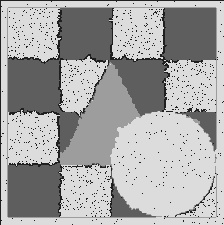
\includegraphics[width=.25\linewidth]{chess_circle_triangle_10.jpg}
\\[\baselineskip]% adds vertical line spacing

\includegraphics[width=.25\linewidth]{tangram_10.jpg}
\\[\baselineskip]% adds vertical line spacing
\caption{EM Segmentation with four/two classes of label}
\end{center}
\end{figure}
\end{frame}

\begin{frame}
\frametitle{EM}
\begin{figure}\label{fg:1}
\begin{center}
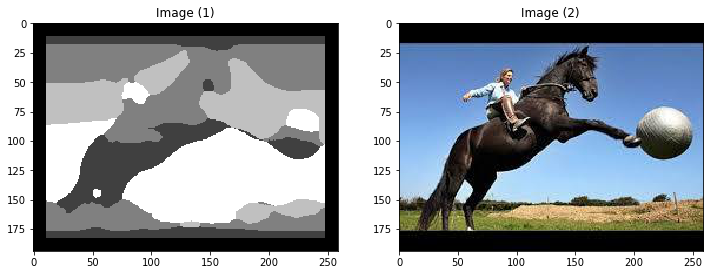
\includegraphics[width=.4\linewidth]{horse_result.png}
\\[\baselineskip]% adds vertical line spacing
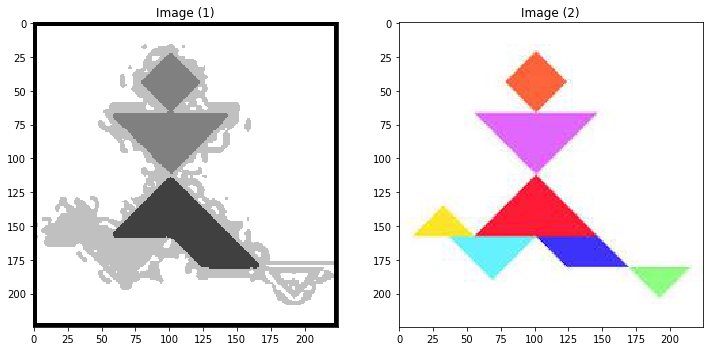
\includegraphics[width=.4\linewidth]{person_result.png}
\\[\baselineskip]% adds vertical line spacing
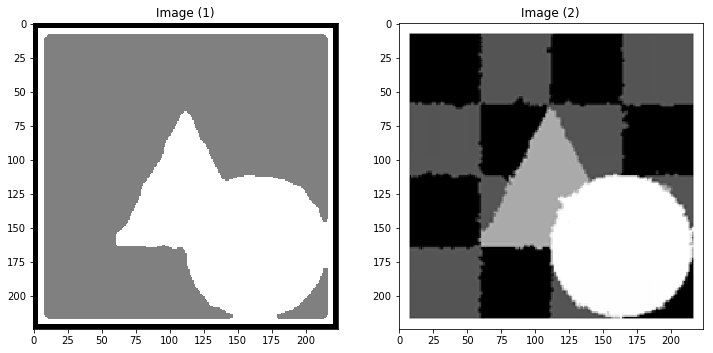
\includegraphics[width=.4\linewidth]{circle_result.png}
\\[\baselineskip]% adds vertical line spacing
\caption{EM Segmentation with four/two classes of label}
\end{center}
\end{figure}
\end{frame}










%------------------------------------------------
%
%\begin{frame}
%
%\bibliographystyle{plainnat}
%\bibliography{reference}
%\end{frame}



%----------------------------------------------------------------------------------------

\end{document}